\section{Introduction}
Local language-model users need correct answers at a lower inference cost. Reusing prior reasoning can improve a reader's observed answer scores, but preparing that reasoning also consumes resources. An accuracy improvement therefore does not establish a cheaper inference pipeline. We examine both the complete token bill and the conditions under which a comparison with direct reading is meaningful, including output allowance, configured context and answer-format rules.

Reasoning reuse offers a concrete way to examine this trade-off. Zou and Tang's Trace as State method places earlier reasoning before the unchanged source, with the question last \citep{tang2026trace}. Its matched control places the same reasoning after the source. Their frontier-model experiments found a placement advantage, while acknowledging additional resource use. Whether that intervention offers a favorable accuracy--cost trade-off on locally served small models remains a separate empirical question.

We address this question through a local reproduction and boundary study on official GraphWalks questions. Two Qwen model packages are tested on the same twelve questions, with five source traces and five reader repeats. We retain the complete graph, archive requests and responses, and charge all source preparation plus one reading when estimating tokens for one answer. Matched trace placements test ordering; comparisons with direct reading examine the larger pipeline. Separate diagnostics check output allowance, configured context and answer-format rules.

The tested configurations did not establish a cost-saving advantage for trace reuse under this single-prediction contract. Both 4B trace placements reached the score ceiling, but a later direct run with a larger output allowance reached the same ceiling with a smaller token bill. The 1.7B placement comparison remained uncertain. Our contribution is evidence about the conditions that a credible low-cost inference comparison must control: a capable direct baseline, full preparation accounting and a qualified evaluation interface. The original placement experiment remains central to that analysis, rather than being replaced by a claim of a new efficient method.

\section{Methods}
\label{sec:migration-contract}
\subsection{Reproduction scope and experimental conditions}
Let $x$ denote the graph context, $q$ its operation, and $T$ a serialized block of prior reasoning. Trace prefix and trace append use $[T,x,q]$ and $[x,T,q]$, respectively. Both receive the same realized $T$ and retain the complete original graph. Direct reading uses $[x,q]$; question-first reading uses $[q,x,q]$. Following the original long-context adaptation of Re2 \citep{tang2026trace,xu2024rereading}, we used $[x,q,x,q]$ within one request. A separate fresh request containing $[x,q]$ is not Re2.

The original study used five source traces and five reader repeats, with each reused trace capped at its first 50,000 characters. All completed short-graph placement studies retained this trace count, repeat count and placement comparison. Their local source and reader output limits were 4,096 and 8,192 tokens, respectively. These explicit local limits differ from the original study, which requested no custom client-side output maximum; effective provider defaults were not established. Appendix~\ref{app:reproduction-map} lists the retained and adapted components.

\paragraph{Tasks and selection.} We used the archived 750-row \protect\path{graphwalks_128k_and_shorter.parquet} file from OpenAI GraphWalks \citep{openai2025graphwalks}, comprising 400 parent and 350 BFS questions. This is one file of the released dataset, not its full repository. Its SHA-256 matched the publisher's current file metadata when checked on 6 October 2026. We used directed breadth-first search (BFS) and parent-retrieval tasks. Gold answers were recomputed from graph edges before scoring. Study-specific selection used catalogue length, task type and exclusion of previously selected graph identities. Earlier selection was deterministic. A separate prospective replication randomly selected six new graphs per task from a restricted short-input population; it was not a random sample of all graph questions. Seeds supplied repeated measurements within graphs and did not increase the number of independent graph units.

\paragraph{Models and interfaces.} The reported studies used the nominal Qwen3-1.7B and Qwen3-4B variants \citep{yang2025qwen3} and Qwen3.5-4B \citep{qwen2026qwen35card}, with native thinking exposed separately from visible answers. The main configurations are listed in Table~\ref{tab:local-configurations}. Model digests, runtime versions, sampling settings and complete prompts are preserved in the frozen archives. Native Qwen3.5 studies used Ollama 0.35.1 and a fixed general-thinking profile. Its temperature was 1.0, top-$p$ 0.95, top-$k$ 20 and presence penalty 1.5. The earlier Qwen3 short-trace study used temperature 0.6, top-$p$ 0.95 and top-$k$ 20. These settings were not pooled as a model-size experiment.

\begin{table}[htbp]
\centering\small
\begin{tabular}{>{\raggedright\arraybackslash}p{.33\linewidth}lll}
\toprule
Study & Model & Context & Source / reader cap\\
\midrule
Initial and prospective short studies & Qwen3-1.7B & 32,768 & 4,096 / 8,192\\
Same-question paired follow-up & Qwen3-4B & 32,768 & 4,096 / 8,192\\
Output-budget diagnostic & Qwen3-4B & 32,768 & --- / 28,672\\
Native source qualification & Qwen3.5-4B & 65,536 & 32,768 / ---\\
Native long five-trace trial & Qwen3.5-4B & 131,072 & 32,768 / 32,768\\
Retained-case context diagnostic & Qwen3.5-4B & 196,608 & retained / 32,768\\
Early-state adaptation & Qwen3.5-4B & 65,536 & 1,024 / budget-derived\\
\bottomrule
\end{tabular}
\caption{Token limits for the main local studies. The early-state reader cap was computed separately for each planned request from its fixed total allowance. Context is a configured serving limit, not a measured guarantee of effective reasoning capacity.}
\label{tab:local-configurations}
\end{table}

\paragraph{Prospective short-graph replication.} Before collecting new responses, we froze a twelve-graph protocol and its complete allocation schedule. All graph heads selected in existing official-study freezes were excluded. Within the catalogue interval $[2000,3500)$ characters, the resulting pools contained 34 parent questions and nine BFS questions with distinct graph heads. Six were sampled without replacement per task, using seed 202610060. Graph order and reader-arm order within each repetition were randomized using the same seeded generator. Five source seeds (202610061--202610065) and five matched reader seeds (202610071--202610075) supplied 240 planned calls. Model digest, original serializer, context and source/reader caps matched the initial short study. Decoding used temperature 0.6, top-$p$ 0.95, top-$k$ 20, minimum-$p$ 0 and repeat penalty 1. The native server version was 0.35.1. Complete requests were saved before transmission and exact response bytes before parsing. No call was retried. Sequential calls were separated by five seconds, and graph blocks by sixty seconds. This was a locally frozen prospective protocol, not an external preregistration.

\paragraph{Same-question second-model follow-up.} After observing the 1.7B results, we froze a separate Qwen3-4B study before collecting its 240 new responses. It retained the same twelve questions, graph and arm order, source and reader seeds, complete prompts, sampling parameters and context/output limits. The 4B package generated its own five-trace bundles. This compared local pipelines on matched questions; it did not isolate reader size or supply twelve additional independent graph units. The within-model prefix--append contrast remained primary, with the same descriptive stratified graph bootstrap.

% BEGIN COMPLETE_DIAGNOSTIC_METHODS
\paragraph{Output-budget diagnostic.} Interim 4B output truncation motivated a separately frozen follow-up on the same twelve known questions and five matched reader seeds. Sixty new direct requests used an output cap of 28,672 tokens, equal to $5\times4096+8192$, with all other recorded inputs, model and sampling settings retained. Original 8,192-cap direct responses remained the historical comparator. This matched maximum generated-token allowances, not total logical tokens, memory, time or compute. Conditions ran sequentially; the diagnostic hypothesis was chosen after interim observations. All cases were retained. The descriptive long-minus-original-direct interval used 20,000 stratified graph-bootstrap draws, seed 202610067.

\paragraph{Configured-context diagnostic.} A separate frozen follow-up retained the original five-trace bundle for the previously declined row-506 case. With the original Qwen3.5-4B digest and sampling profile, it changed the configured context from 131,072 to 196,608 tokens. One full-prefix input probe with a one-token output cap checked accounting and residency without scoring an answer. Five paired seeds supplied prefix, append, fresh, question-first and Re2 readers, each with a 32,768-token output cap: 26 new calls in total. Five-second call gaps and sixty-second repeat-block rests were retained. Full original source preparation was charged to trace conditions; new-run usage was separately reported. This deliberately selected failure case diagnosed execution and case-specific outcomes, not a new population sample or completion of the old sixteen-graph trial.

% END COMPLETE_DIAGNOSTIC_METHODS

\paragraph{Trace construction and controls.} Source reasoning was read from the native thinking field; the separate visible answer was excluded. Incorrect and length-terminated source traces were retained according to each frozen protocol. Prefix and append used byte-identical trace blocks. The shorter-state adaptation retained the complete thinking generated under a 1,024-token cap. It did not select excerpts using gold answers. Representation recoding and thinking-mode controls were separate experiments, reported in the appendices.

\subsection{Scoring, qualification and missing outcomes}
For predicted and gold node sets $P$ and $G$, we used
\[
 F_1(P,G)=\begin{cases}
 1,&P=G=\varnothing,\\
 \displaystyle\frac{2|P\cap G|}{|P|+|G|},&\text{otherwise},
 \end{cases}
 \qquad \mathrm{EM}(P,G)=\mathbf{1}\{P=G\}.
\]
Set semantics remove duplicate predictions but retain incorrect nodes. Scoring used visible answers only and never extracted an answer from thinking. Known malformed or length-terminated outputs received zero under their respective protocols. Valid empty answers were scored normally, with an always-empty baseline reported where relevant.

\paragraph{Answer interfaces.} The native source and configured-context studies accepted a valid terminal visible \texttt{Final Answer: [...]} line after a normal stop. The early-state study required that line to constitute the entire visible response. Its later relaxed parser was explicitly post hoc and did not replace the primary scores. Recoding protocols also differed in their treatment of unmapped nodes. Identity recoding invalidated such predictions, whereas indexed-source scoring counted them as false positives. Scores were not pooled across these rules.

\paragraph{Call qualification.} Input counts, response metadata and resident model digest/context were checked against the recorded request. Qualification established compliance with the study's interface, not answer correctness. A qualified response could still be malformed or reach its output limit. A returned response that failed interface qualification remained undetermined under the applicable primary protocol.

\paragraph{Interrupted execution.} Unknown responses were bounded over the original planned denominator, rather than scored as zero or replayed. For $N$ planned outcomes with $m$ unknown values, the F1 bounds were $[\sum F_1/N,(\sum F_1+m)/N]$. Known unsent budget declines were deployment failures, not model answers. Client errors retained their protocol-defined failure scores and unknown usage. Unknown token usage made the reported cost a lower bound.

\subsection{Statistical analysis and resource accounting}
Reader repetitions were averaged within graphs before comparisons across graphs. Intervals condition on the archived trace bundles; independent redraws of complete five-trace bundles were not sampled. The short-trace study used 20,000 graph bootstrap resamples, seed 202610040, for descriptive 95\% percentile intervals. Its four graphs did not support a broad population claim. The twelve-graph replication specified prefix-minus-append F1 as its primary contrast and prefix-minus-direct as secondary. Each task stratum contributed equally. Its descriptive percentile intervals used 20,000 bootstrap draws of six graph units within each task stratum, seed 202610066. All twelve selected graphs and all repeated outcomes were included, without score-dependent stopping. Subsequent studies retained their own frozen analysis families and screening criteria (Appendix~\ref{app:gate-map}). These criteria governed advancement to further research; they were not universal definitions of successful replication or formal noninferiority tests.

Deployment-token accounting included the complete source inputs and outputs plus one reader's input and output. Repeated reader calls estimated that reader cost; they did not divide the preparation bill. Research-run totals were reported separately and included calibration where performed. Token accounting did not establish latency, energy or cache-related computation savings. The prospective replication separately recorded observed request wall times, without an exclusive-hardware or comparative-latency claim. A dedicated API endpoint also did not establish exclusive hardware use. No existing protocol, response or primary score was changed during the manuscript revision.

\section{Results}
\label{sec:migration-results}
\subsection{Prospective replication left the placement advantage uncertain}
\label{sec:prospective-replication}
The twelve-graph follow-up completed all 240 planned calls: sixty sources and sixty reader responses per condition. Every call passed the recorded interface checks; none was declined for context or had unknown usage. Twelve sources reached their 4,096-token limit. Prefix and append each produced sixty normal-valid visible answers, compared with 59 for direct reading; the remaining direct response reached its output limit. Incorrect and truncated source reasoning remained in the shared trace block.

Mean F1 was 0.7715 for prefix, 0.7351 for append and 0.6915 for direct reading (Figure~\ref{fig:prospective-replication}). The primary prefix-minus-append difference was 3.64 percentage points, with a descriptive interval of $[-0.65,8.33]$ points. The secondary prefix-minus-direct difference was 8.00 points, interval $[-3.00,17.98]$ points. Both intervals included zero. EM was 0.3333, 0.3833 and 0.3333 respectively: the higher prefix F1 did not extend to exact match. Two graphs had empty gold answers; an always-empty response therefore scored 0.1667 in both metrics over this sample.

The prefix-minus-direct F1 point difference was $+20.79$ points for parents but $-4.80$ points for BFS. These six-graph strata did not establish a task-specific causal mechanism. They showed why an aggregate positive point estimate should not be described as a uniform improvement. The follow-up remained separate from the initial four graphs; their scores and intervals were not pooled.

Charging all five source calls plus one seed-averaged reading gave mean deployment costs of 34,901.15 tokens for prefix, 34,622.07 for append and 4,093.48 for direct reading. Prefix cost $8.53$ times direct reading under this single-question contract. The complete research run consumed 2,308,239 model tokens. Observed request wall times summed to 4,115.32 seconds, excluding the planned idle gaps; this was neither total elapsed deployment time nor a hardware-exclusive latency comparison.

\begin{figure}[htbp]
\centering
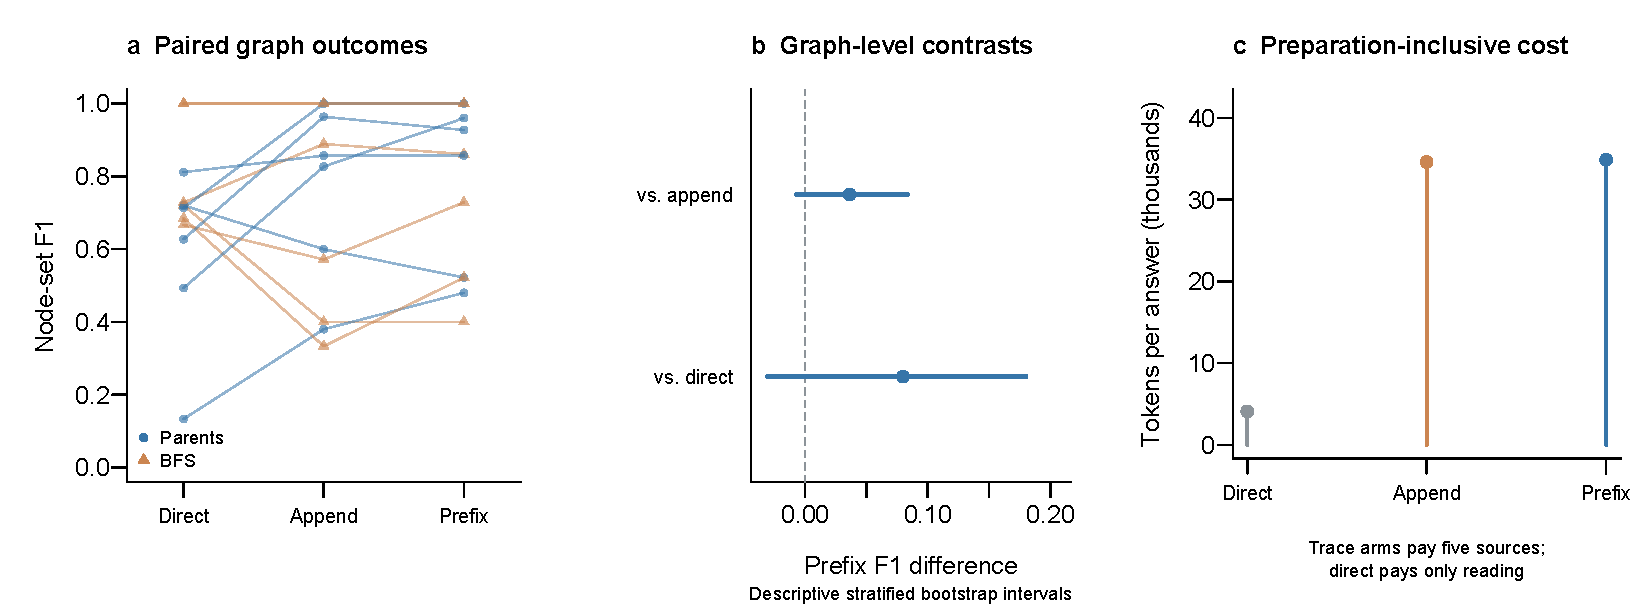
\includegraphics[width=\linewidth]{figures/official_graph_confirmatory_20261006.pdf}
\caption{Prospective twelve-graph replication, drawn in R from independently rescored raw responses. (a) Paired per-graph F1 means over five reader seeds, with six parent and six BFS questions. (b) Primary and secondary prefix contrasts with descriptive stratified graph-bootstrap intervals. (c) Mean tokens for one answer: trace conditions pay all five source calls and one seed-averaged reader; direct pays only the reader. All 240 calls completed, and failures of output format or termination retain their prespecified zero scores. The two empty-answer graphs remain in all analyses.}
\label{fig:prospective-replication}
\end{figure}

% BEGIN COMPLETE_PAIRED_NUMERIC_TABLE
\begin{table}[htbp]
\centering\small
\begin{tabular}{lrrrr}
\toprule
Configuration & F1 & EM & Normal-valid & Tokens/answer\\
\midrule
1.7B prefix & 0.7715 & 0.3333 & 60/60 & 34,901\\
1.7B append & 0.7351 & 0.3833 & 60/60 & 34,622\\
1.7B direct & 0.6915 & 0.3333 & 59/60 & 4,093\\
4B prefix & 1.0000 & 1.0000 & 60/60 & 51,751\\
4B append & 1.0000 & 1.0000 & 60/60 & 51,612\\
4B direct & 0.6967 & 0.6833 & 42/60 & 8,231\\
\bottomrule
\end{tabular}
\caption{Completed Qwen3 comparisons on the same twelve graphs, five reader repeats each. Trace costs charge all five sources and one reader. Normal-valid refers to termination and visible-answer format, not correctness. The same questions are not twenty-four independent graph units.}
\label{tab:paired-final}
\end{table}


% END COMPLETE_PAIRED_NUMERIC_TABLE

\subsection{The second model reached a ceiling in both trace placements}
\label{sec:paired-models}
The same-question Qwen3-4B follow-up completed all 240 planned calls and passed independent request, token-count, runtime and scoring checks. Prefix and append each gave sixty normal-valid and exact answers: mean F1 and EM were both 1.0000 (Figure~\ref{fig:paired-models}). All sixty source calls reached the 4,096-token limit and therefore had zero visible-answer scores. Their thinking was nevertheless retained according to the frozen rule. Successful second-pass answering with supplied traces did not require a completed correct visible source answer under this budget.

Direct reading achieved F1 0.6967 and EM 0.6833. Eighteen of sixty direct responses reached the 8,192-token limit; forty-two stopped normally with valid terminal answers. Prefix minus direct F1 was 30.33 percentage points, with a descriptive interval of $[13.67,46.67]$ points. The task-stratum differences were $+0.67$ points for parents and $+60.00$ points for BFS. This pipeline contrast included additional reasoning, warning instructions and preparation calls, and could be affected by direct-output truncation. It did not isolate a placement effect or a same-total-budget advantage.

The primary prefix--append contrast was exactly zero on every graph. Its bootstrap interval collapsed to zero because both conditions were at the observed score ceiling, not because population equivalence had been established. The supplied-trace conditions answered these questions reliably, while leaving no observed preference for front placement. This observation did not by itself establish how the reader used the traces. Cross-model differences also included separately generated trace content, rather than reader size alone.

Preparation-inclusive mean tokens per answer were 51,751.22 for prefix, 51,611.63 for append and 8,231.05 for direct reading. Prefix required $6.29$ times the direct tokens. The complete research run used 3,740,754 model tokens; observed request-wall times summed to 15,435.86 seconds, excluding planned rests. These were logical usage and observed timings, not energy or hardware-exclusive latency measurements.

\begin{figure}[htbp]
\centering
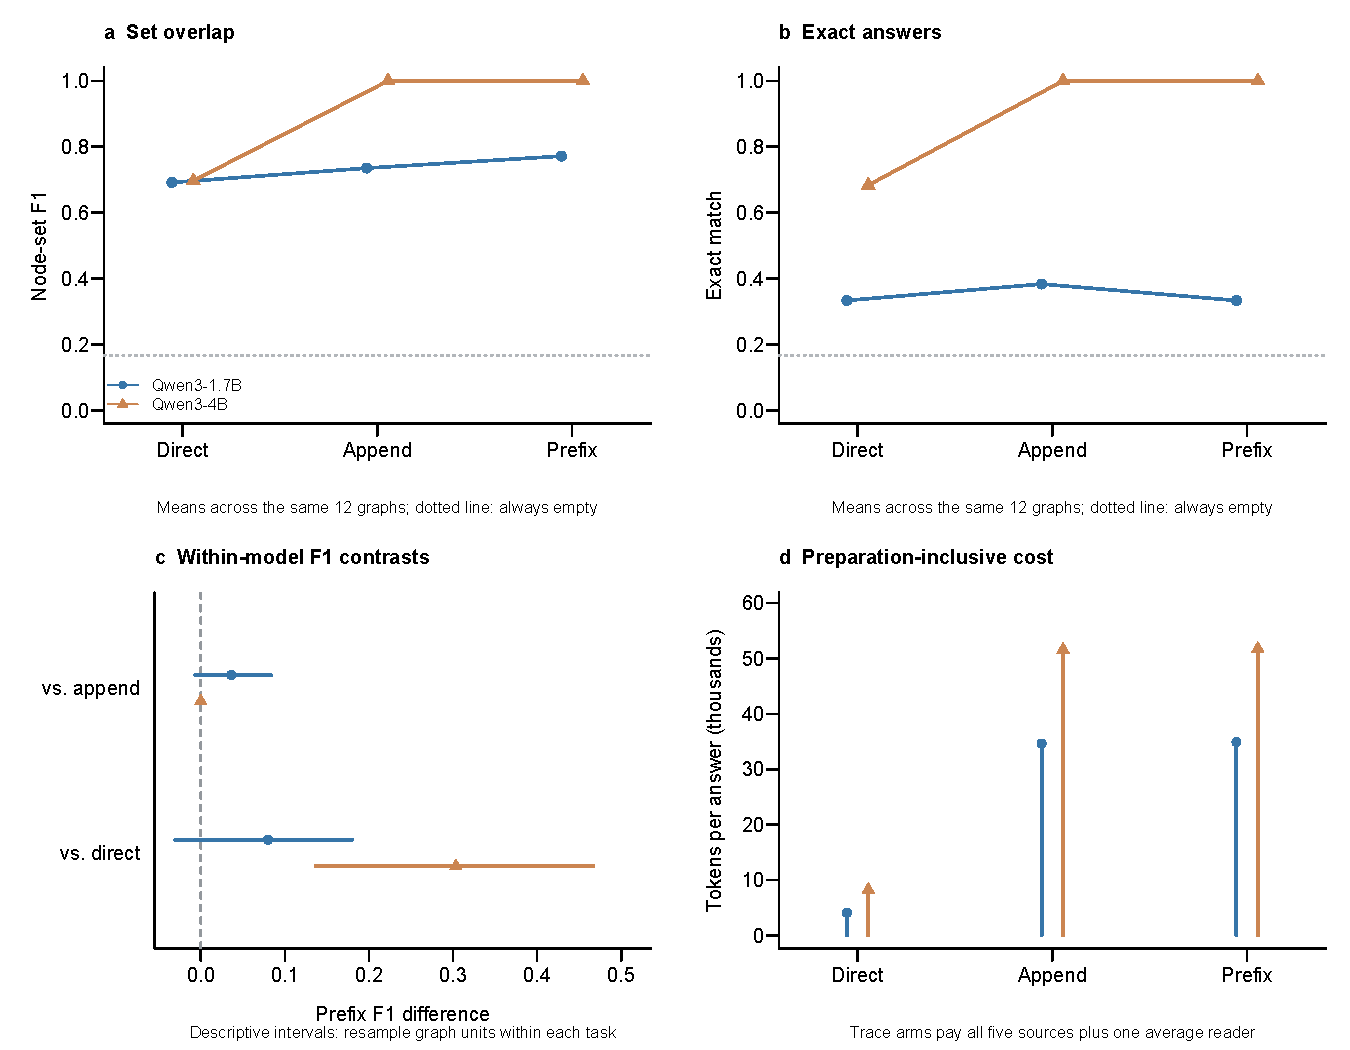
\includegraphics[width=\linewidth]{figures/paired_models_20261006.pdf}
\caption{Local Qwen3 configurations on the same twelve questions, rendered in R from two independently audited 240-call studies. (a,b) F1 and exact-match means; the dotted line is the always-empty baseline. (c) Within-model prefix contrasts with descriptive stratified graph-bootstrap intervals. The zero-width 4B prefix--append interval reflects an observed ceiling, not population equivalence. (d) Tokens for one answer, charging all five sources for trace conditions. Model packages generate their own traces; this is not a size-only comparison. Eighteen 4B direct answers were length-terminated and retained their prescribed zero scores.}
\label{fig:paired-models}
\end{figure}

% BEGIN COMPLETE_OUTPUT_BUDGET_RESULTS
\subsection{A larger output allowance was tested on the same questions}
\label{sec:output-budget}
All sixty new direct-long calls completed and passed independent request and scoring checks. With a 28,672-token output cap, mean F1 was 1.0000, EM 1.0000, and 60/60 responses were normal-valid. There were 0 length-terminated outputs, compared with eighteen under the original cap. The paired F1 change from the original direct condition was 30.33 percentage points, with a descriptive interval of $[13.33,46.67]$ points. These results quantify this sequential diagnostic on the known questions, rather than a fresh-case or equal-compute comparison.

Mean logical tokens for one direct-long answer were 8,763.78, compared with 8,231.05 in the original direct condition. The new diagnostic incurred 525,827 model tokens and 5,912.53 seconds of observed request time, excluding planned rests. The original trace scores and costs were not overwritten. Prefix preparation cost was 5.91 times direct-long tokens, with the same observed F1 and EM ceiling.

Among the eighteen previously length-terminated responses, 0/18 new thinking strings began with the old thinking text with trailing whitespace removed. The new runs were therefore not byte-identical continuations of the old runs despite matching seeds. This descriptive check further limits attribution of every changed answer to the output cap alone.

\begin{table}[htbp]
\centering\small
\begin{tabular}{lrrrr}
\toprule
Output cap & F1 & EM & Normal-valid & Tokens/answer\\
\midrule
8192 & 0.6967 & 0.6833 & 42/60 & 8,231\\
28672 & 1.0000 & 1.0000 & 60/60 & 8,764\\
\bottomrule
\end{tabular}
\caption{Sequential Qwen3-4B diagnostic on the same known questions and seeds. The larger cap equals the five-source pipeline maximum generated-token allowance, not its total logical-token or compute budget. Original 8192-cap responses remain unchanged.}
\label{tab:budget-final}
\end{table}


\begin{figure}[htbp]
\centering
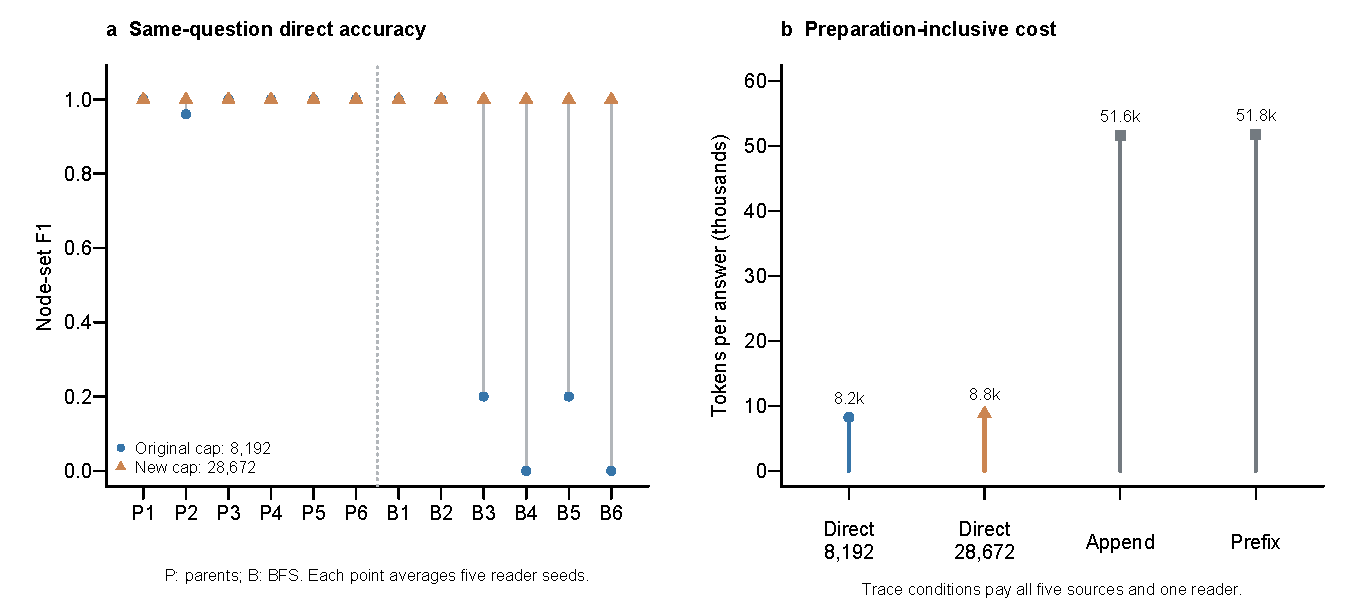
\includegraphics[width=\linewidth]{figures/output_budget_20261006.pdf}
\caption{Output-budget diagnostic on the same twelve Qwen3-4B questions, rendered in R from complete independent audits. (a) Direct F1 averaged over five seeds per graph, with parents and BFS displayed separately. Old length-terminated responses retain zero scores. (b) Mean logical tokens for one answer; trace conditions charge all five sources. New direct answers and both trace placements reached the observed F1/EM ceiling. The sequential known-question diagnostic matches maximum generated allowances, not total compute, and does not establish population equivalence or isolated causality.}
\label{fig:output-budget}
\end{figure}

% END COMPLETE_OUTPUT_BUDGET_RESULTS

\subsection{Native source qualification succeeded on the selected graphs}
A separately frozen Qwen3.5-4B experiment tested source answering with a larger context and output allowance. Earlier bridge archives are retained for selection lineage but excluded from empirical claims because their transmitted-request provenance is weaker (Appendix~\ref{app:reproduction-map}).

With a 65,536-token context and 32,768-token source output cap, all sixteen source calls stopped normally and met qualification. Across eight new graphs, F1 was 0.9286 and EM was 0.875. Figure~\ref{fig:hybrid-source} shows that errors remained on a long-BFS graph. The source screening criterion passed, providing a qualified starting point for the next migration trial. These calls did not test second-pass trace reuse.

\begin{figure}[htbp]
\centering
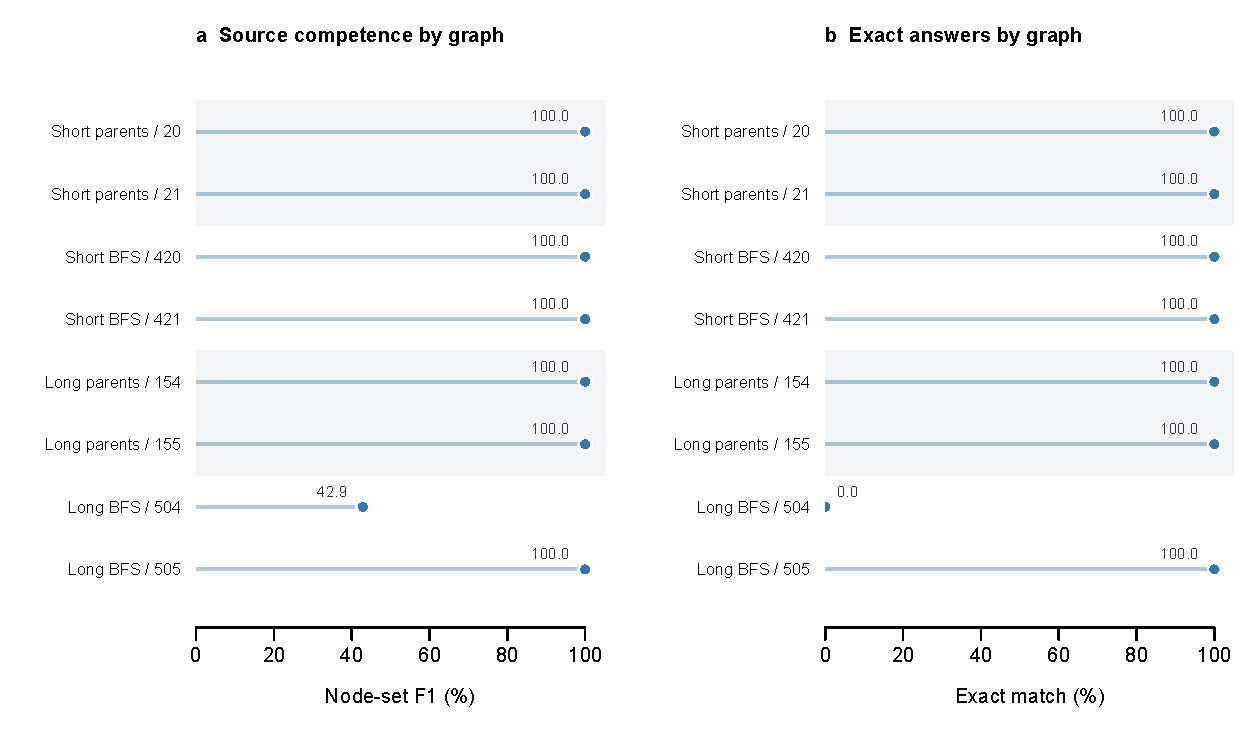
\includegraphics[width=0.92\linewidth]{figures/source_qualification_figure.pdf}
\caption{Native source performance on eight official graphs. Each dot is a graph mean over two seeds; row identifiers locate the released questions. F1 and exact match are shown separately. No inferential error bars are shown for this source-qualification study. All empirical panels were drawn in R from audited CSV inputs.}
\label{fig:hybrid-source}
\end{figure}

\subsection{Five native traces exceeded the configured reader context}
The next trial planned sixteen long-BFS graphs, five sources per graph and five repeats of five reader conditions. On the first graph, prefix and append each required 144,677 input tokens. This exceeded the configured 131,072-token context before any reader output was generated (Figure~\ref{fig:hybrid-interrupted}). Both trace conditions were declined under the frozen resource rule, without shortening their trace block.

The trial subsequently stopped after a returned response failed its resident-model check. Of 480 planned formal slots, fourteen returned qualified responses, eight were budget declines, one returned response was unqualified, and 457 were unreached. These categories preserved 22 determined deployment outcomes and 458 unknown outcomes. The archive established first-graph infeasibility under the specified configuration, but not a sixteen-graph quality effect.

The frozen inputs also permitted a conditional cost calculation. Let $I$ be one complete source input and $C$ the direct output allowance. Five source inputs alone cost $5I$, whereas one direct prediction costs at most $I+C$. Hence
\[
 I>C/4\quad\Longrightarrow\quad 5I>I+C.
\]
All sixteen planned inputs satisfied $I>8192$ with $C=32768$. Under this single-prediction accounting contract, five complete sources could not be cheaper than direct reading. This bound did not apply to latency, caching, different output caps or preparation reused across different questions.

\begin{figure}[htbp]
\centering
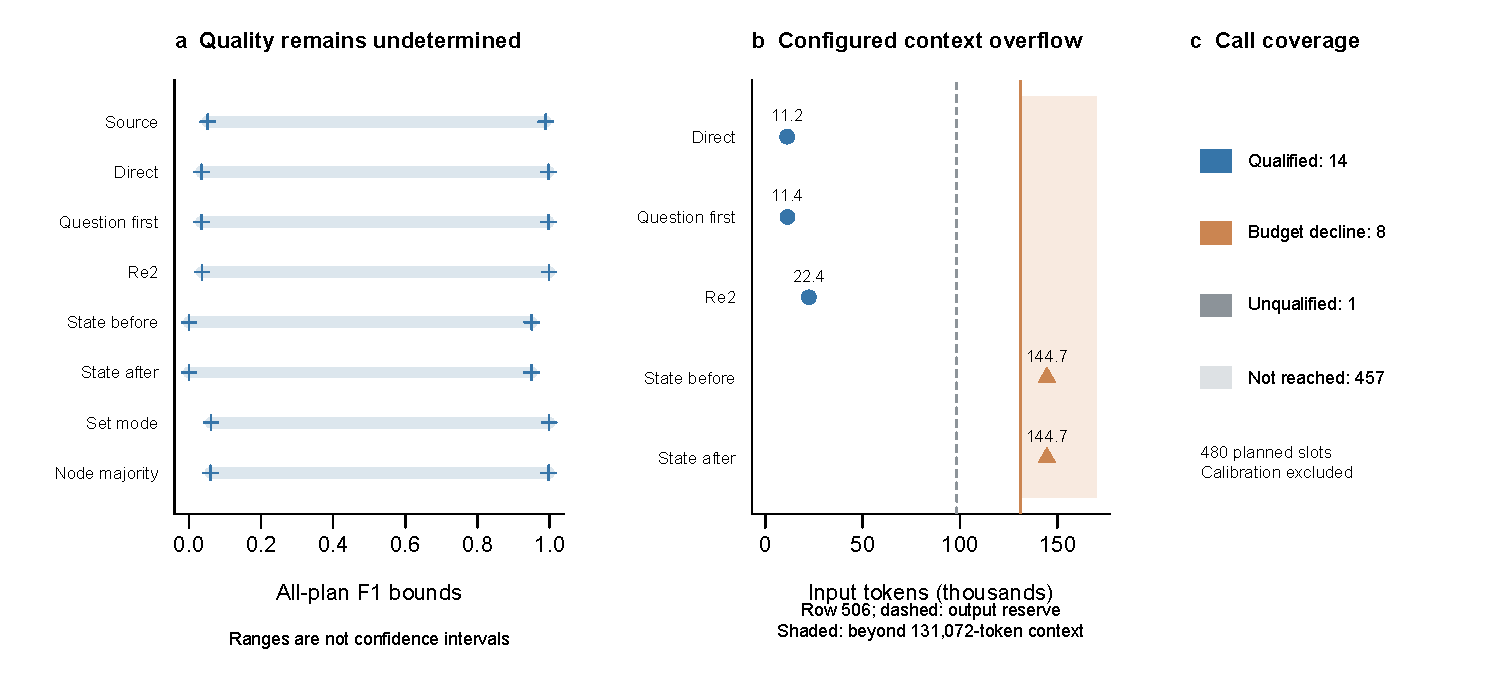
\includegraphics[width=\linewidth]{figures/interrupted_study_figure.pdf}
\caption{Context and execution boundaries in the native five-trace trial. (a) F1 identification bounds retain all sixteen planned graph outcomes; they are not confidence intervals. (b) First-graph rendered inputs, with the configured context marked by a solid line and the input limit after output reservation by a dashed line. (c) Coverage of 480 formal slots, excluding calibration. Budget declines and unreached slots are distinct from returned answers.}
\label{fig:hybrid-interrupted}
\end{figure}

% BEGIN COMPLETE_CONTEXT_DIAGNOSTIC_RESULTS
\subsection{A larger configured context enabled the retained-case diagnostic}
\label{sec:context-diagnostic}
All twenty-six new calls passed independent request, input-count and resident-model checks at a configured 196,608-token context. The probe verified the full 144,677-token prefix input; it was not a scored answer. This established execution at the changed allocation for this case, rather than reasoning capacity throughout the context window.

Across five reader seeds, prefix F1/EM were 0.9750/0.8000, append 0.8984/0.6000, and fresh direct reading 0.9583/0.4000. Normal-valid counts were 5/5, 5/5 and 5/5 respectively. Table~\ref{tab:context-final} retains all five conditions. No population interval was inferred from this deliberately selected case. The old sixteen-graph archive remained interrupted and its unknown outcomes were not replaced.

The original five-source preparation cost was 190,884 tokens. New probe and reader calls consumed 2,343,997 model tokens, with 12,135.52 seconds of observed request time. Preparation was charged once to each trace deployment estimate, never amortized over the five experimental repeats.

\begin{table}[htbp]
\centering\small
\begin{tabular}{lrrrr}
\toprule
Reader & F1 & EM & Normal-valid & Tokens/answer\\
\midrule
prefix & 0.9750 & 0.8000 & 5/5 & 350,021\\
append & 0.8984 & 0.6000 & 5/5 & 344,816\\
fresh & 0.9583 & 0.4000 & 5/5 & 36,498\\
question first & 0.7220 & 0.0000 & 5/5 & 39,719\\
re2 & 0.7692 & 0.6000 & 4/5 & 50,578\\
\bottomrule
\end{tabular}
\caption{One previously selected overflow case, evaluated at a configured 196608-token context with the original trace bundle. Five repeats per condition describe this case only; no population interval is inferred. Prefix and append include the complete original source preparation cost.}
\label{tab:context-final}
\end{table}


% END COMPLETE_CONTEXT_DIAGNOSTIC_RESULTS

\subsection{Answer-format sensitivity limited the early-state comparison}
A separately frozen adaptation used a 1,024-token source cap and seven reader conditions with a shared total-token allowance. Execution remained incomplete, with 129 of 224 planned reader outcomes known. Under a post hoc parser that accepted a valid terminal answer within surrounding prose, prefix, direct and question-first reading each produced thirteen exact answers on eighteen matched outputs. The primary strict scores were retained. This sensitivity showed that an apparent strict-score advantage could depend on format compliance; it did not establish equivalence or a placement benefit. Appendix~\ref{app:early-state-detail} reports the planned-denominator bounds, failures and resource accounting.

\subsection{Additional controls identified separate sources of variation}
The initial four-graph Qwen3-1.7B study also favored prefix in mean F1, but both paired descriptive intervals included zero. Appendix~\ref{app:initial-short-study} retains its full numerical results and preparation cost; it is not pooled with the prospective twelve-graph follow-up.

Representation and decoding studies tested interventions distinct from trace placement. Reversible compact node names improved the F1 point estimate by 15.23 points and reduced tokens by 50.46\%. Its eight-graph interval against original names was $[-21.15,40.98]$ points, leaving the quality effect uncertain. Thinking-off and a fixed task route reduced tokens while lowering quality (Appendix~\ref{app:representation-controls}).

The indexed-source study saved 94 of 96 planned responses. Its primary indexed-off candidate failed the frozen criterion. A secondary compact-on comparison remained positive under worst-case missing-score bounds, but unknown usage prevented a complete cost comparison (Appendix~\ref{app:indexed-source}). Small longer-input and sampling studies also showed sensitivity to decoding and empty-answer baselines. They did not identify a single causal sampling parameter or a universal long-input failure.

\section{Discussion}
The local experiments did not establish that preparing and reusing reasoning lowered the token cost of one accurate answer. This deployment question must be separated from whether supplying traces improves an answer under a particular reader cap. The initial and prospective Qwen3-1.7B studies favored trace prefix in mean F1, but both descriptive placement intervals included zero. The twelve-graph study also showed lower prefix EM than append and opposing prefix-versus-direct point differences across tasks. On the same questions, Qwen3-4B reached perfect F1 and EM in both trace placements; its direct condition was substantially affected by output truncation. Thus answering with supplied traces and a front-placement advantage were different empirical questions. The native source study showed that selected graph questions could be answered reliably under a different configuration. It did not establish that a reader would benefit from those traces.

% BEGIN COMPLETE_DIAGNOSTIC_DISCUSSION
In the output-budget diagnostic, direct F1 was 1.0000 versus 0.6967 in the earlier run, with the same questions and sampling settings. The prefix preparation-inclusive token bill was 5.91 times that of the new direct condition at the same observed accuracy ceiling. Because its hypothesis was selected after truncation and conditions ran sequentially, it supports a bounded output-budget interpretation, not a pure causal estimate of the reasoning-state mechanism. The retained-case context diagnostic also separated a configured allocation failure from execution at a larger allocation; it did not fill the old trial's missing quality outcomes.

% END COMPLETE_DIAGNOSTIC_DISCUSSION

\paragraph{Relation to Trace as State.} The original method supplies prior reasoning before an unchanged source, allowing it to guide rereading \citep{tang2026trace}. Our placement comparison retained that intervention. Differences in models, task lengths, output limits and interfaces prevented a direct comparison with the original benchmark scores. The local uncertainty therefore did not contradict the reported frontier-model result. The original paper also acknowledged additional latency and token costs; our accounting quantified a particular local configuration rather than identifying a flaw overlooked by its authors.

\paragraph{Separating the constraints.} Source competence, reader feasibility and placement benefit are distinct questions. A successful source pass answers only the first. Conversely, an incorrect or incomplete source answer does not rule out useful intermediate reasoning: source correctness is not a prerequisite for testing reuse. Context overflow prevents the second pass from testing placement at all. Output-format sensitivity limits interpretation of a measured score difference. Treating these conditions separately prevents an execution failure or parsing difference from being mistaken for a failure of the underlying reasoning principle.

\paragraph{Implications for low-cost inference.} In these graph configurations, the larger-output direct diagnostic achieved the same observed 4B accuracy ceiling as the trace conditions with a smaller preparation-inclusive token bill. This is a sequential, known-question diagnostic, not an equal-compute or purely causal comparison. It motivates checking whether a direct baseline has sufficient output allowance before attributing a pipeline advantage to reuse. A lower-cost trace pipeline would also need to reduce or amortize its preparation; the present traces were question-specific, and cross-question amortization was not measured. Token usage does not by itself establish latency, energy or monetary savings.

\paragraph{Implications for further reproduction.} Further long-input reproduction should first ensure that the intended trace block and output reserve fit every selected input. It should then compare identical trace content before and after the source with paired graph measurements. Semantic correctness, strict output compliance and truncation should be specified separately before collection. Fewer traces or compressed traces change the intervention and require their own matched controls. These are prospective requirements, not additional findings of this study.

\paragraph{Contribution of the boundary study.} The primary contribution is a local accuracy--cost assessment grounded in a reproduction of the placement intervention. The evidence identifies qualified source configurations, cases where the intended second pass was declined under its configured resource contract, and a scoring confound requiring explicit control. It narrows the conditions for a meaningful small-model test. Representation changes and source-free experiments remain exploratory extensions, separate from the placement evidence.

\section{Limitations}
The initial placement study used four graphs with deterministic selection. The prospective follow-up used twelve randomized graph units from restricted, previously unselected short-input pools, including only nine eligible BFS graph heads before sampling. Five readings of each graph did not create additional independent graph units. Most other study selections remained deterministic. The results cannot estimate general performance across tasks, models or domains. Unused graph identities were new to this workflow, not established as absent from model pretraining; public-benchmark contamination was not assessed. Native long-trace and early-state trials were interrupted, so their full-sample quality effects remained unknown. Model families, input complexity and decoding settings changed between studies, preventing architecture-only or scale-only attribution.

Graph questions admit exact conventional algorithms. They served as controlled probes of model behavior, not evidence that language models outperform graph parsers. Legacy synthetic and document experiments had different protocols and incomplete response provenance; they were excluded from the primary evidence. Local hashes and recorded runtime snapshots support consistency checks but do not prove continuous exclusive hardware use or third-party execution authenticity. Token counts alone do not establish energy, monetary or latency savings.

The source traces were prepared for each evaluated question; cross-question reuse and question-independent compression were not tested. The prefix--append contrast holds trace content and its warning wrapper fixed and tests placement. Comparisons with direct reading additionally change supplied content, instructions and preparation compute; they do not isolate a latent-state mechanism or a same-total-budget gain. The incomplete early-state controls cannot remove these ambiguities from the completed five-trace studies.

\section{Conclusion}
We evaluated reasoning reuse as a candidate for lower-cost local inference by reproducing the Trace as State placement intervention and accounting for complete preparation. The tested configurations did not establish a cost-saving or placement-specific advantage. A larger-output direct 4B diagnostic reached the same accuracy ceiling as trace reuse with a smaller token bill, while context fit and answer-format rules constrained other comparisons. Credible efficiency claims therefore require a capable direct baseline, explicit preparation costs and a qualified evaluation interface. These findings apply to the tested graph configurations and single-prediction accounting contract; they do not establish a universal deployment rule.
